\documentclass[11pt]{article}

% Change "review" to "final" to generate the final (sometimes called camera-ready) version.
% Change to "preprint" to generate a non-anonymous version with page numbers.
\usepackage[final]{acl}

% Standard package includes
\usepackage{times}
\usepackage{latexsym}

% For proper rendering and hyphenation of words containing Latin characters (including in bib files)
\usepackage[T1]{fontenc}
% For Vietnamese characters
% \usepackage[T5]{fontenc}
% See https://www.latex-project.org/help/documentation/encguide.pdf for other character sets

% This assumes your files are encoded as UTF8
\usepackage[utf8]{inputenc}

\usepackage{booktabs}
\usepackage{tabularx}

% This is not strictly necessary, and may be commented out,
% but it will improve the layout of the manuscript,
% and will typically save some space.
\usepackage{microtype}

% This is also not strictly necessary, and may be commented out.
% However, it will improve the aesthetics of text in
% the typewriter font.
\usepackage{inconsolata}

%Including images in your LaTeX document requires adding
%additional package(s)
\usepackage{graphicx}

\usepackage{array}
\usepackage{amsmath}
\usepackage{placeins}

% defined commands:
\newcommand{\method}[1]{\textbf{M#1}}
\newcommand{\nr}{\mathrm{NR}}

% If the title and author information does not fit in the area allocated, uncomment the following
%
%\setlength\titlebox{<dim>}
%
% and set <dim> to something 5cm or larger.

\title{What is the price of a model's eye?:\\ Understanding How VLMs Answer Multiple Choice Questions in Multimodal Settings}

% Author information can be set in various styles:
% For several authors from the same institution:
% \author{Author 1 \and ... \and Author n \\
%         Address line \\ ... \\ Address line}
% if the names do not fit well on one line use
%         Author 1 \\ {\bf Author 2} \\ ... \\ {\bf Author n} \\
% For authors from different institutions:
% \author{Author 1 \\ Address line \\  ... \\ Address line
%         \And  ... \And
%         Author n \\ Address line \\ ... \\ Address line}
% To start a separate ``row'' of authors use \AND, as in
% \author{Author 1 \\ Address line \\  ... \\ Address line
%         \AND
%         Author 2 \\ Address line \\ ... \\ Address line \And
%         Author 3 \\ Address line \\ ... \\ Address line}

% For several authors from the same institution:
\author{Divyanshu Giri, Rachit Mehta, Yashav Bhatnagar \\
        IIIT Hyderabad}

% \author{Divyanshu Giri \\
%   Affiliation / Address line 1 \\
%   Affiliation / Address line 2 \\
%   Affiliation / Address line 3 \\
%   \texttt{divyanshu.giri@research.iiit.ac.in} \\\And
%   Rachit Mehta \\
%   Affiliation / Address line 1 \\
%   Affiliation / Address line 2 \\
%   Affiliation / Address line 3 \\
%   \texttt{rachit.mehta@students.iiit.ac.in} \\}

%\author{
%  \textbf{First Author\textsuperscript{1}},
%  \textbf{Second Author\textsuperscript{1,2}},
%  \textbf{Third T. Author\textsuperscript{1}},
%  \textbf{Fourth Author\textsuperscript{1}},
%\\
%  \textbf{Fifth Author\textsuperscript{1,2}},
%  \textbf{Sixth Author\textsuperscript{1}},
%  \textbf{Seventh Author\textsuperscript{1}},
%  \textbf{Eighth Author \textsuperscript{1,2,3,4}},
%\\
%  \textbf{Ninth Author\textsuperscript{1}},
%  \textbf{Tenth Author\textsuperscript{1}},
%  \textbf{Eleventh E. Author\textsuperscript{1,2,3,4,5}},
%  \textbf{Twelfth Author\textsuperscript{1}},
%\\
%  \textbf{Thirteenth Author\textsuperscript{3}},
%  \textbf{Fourteenth F. Author\textsuperscript{2,4}},
%  \textbf{Fifteenth Author\textsuperscript{1}},
%  \textbf{Sixteenth Author\textsuperscript{1}},
%\\
%  \textbf{Seventeenth S. Author\textsuperscript{4,5}},
%  \textbf{Eighteenth Author\textsuperscript{3,4}},
%  \textbf{Nineteenth N. Author\textsuperscript{2,5}},
%  \textbf{Twentieth Author\textsuperscript{1}}
%\\
%\\
%  \textsuperscript{1}Affiliation 1,
%  \textsuperscript{2}Affiliation 2,
%  \textsuperscript{3}Affiliation 3,
%  \textsuperscript{4}Affiliation 4,
%  \textsuperscript{5}Affiliation 5
%\\
%  \small{
%    \textbf{Correspondence:} \href{mailto:email@domain}{email@domain}
%  }
%}

\begin{document}
\maketitle
\begin{abstract}
MCQA is a key competence of vision-language models that is tested by a variety of mainstream benchmarks. However, these models can have a wide range of changes in performance when the task is diversified even slightly. The question we are asking is: \textit{how do mainstream vision-language models perform on formatted multiple-choice question answering tasks?} Using a counterfactual dataset derived from CLEVR scenes,  we set out to evaluate and understand the models' internal representations by employing methods like layer-wise activation patching, individual attention head localization, and vocabulary projection for answer choices to localize key hidden states and activation patterns that encode information about predictive tokens. Our experiments so far suggest that visual information is available early in image tokens, passes through option-content semantic representations in the middle layers, and reach the answer position and symbols in the late layers, mainly through attention. We find that all answer labels show a late increase in the logits, while a sparse set of attention heads separates the correct label. We also observe that common answer alphabets are more robustly promoted in vocabulary space than rare symbols. Our ongoing work will extend this analysis to other model families and to vision specific experiments separating visual-grounding features from symbol-binding features if time permits.
\end{abstract}

\section{Introduction}

Multi-choice question answering (MCQA) has been a popular task for evaluating LMs \cite{wiegreffe2025answerassembleaceunderstanding}, and has been gaining traction in the space of vision-language models recently \cite{meng2024mmiumultimodalmultiimageunderstanding}. A prominent example is the MMMU benchmark \cite{yue2024mmmumassivemultidisciplinemultimodal} and its successor \cite{yue2025mmmuprorobustmultidisciplinemultimodal} which evaluates multimodal models on massive multi-discipline tasks on a large number of open-source LMMs as well as proprietary models. While LMs have been evaluated comprehensively in this domain, VLMs are yet to be probed in depth. In fact, its successor \cite{yue2025mmmuprorobustmultidisciplinemultimodal}, removes the questions that text-only models can answer, expands the number of answer choices and adds a vision-only setting, under which the performance of VLMs dropped significantly. At the same time, prior work shows that text-only models are not robust to seemingly inconsequential format changes, such as shuffling the position of the correct answer or changing the symbols the answers are mapped to \cite{wiegreffe2025answerassembleaceunderstanding}.

Our focus is not on whether the model answers correctly but on which layer and which attention heads produce that answer. While benchmarks like MMLU and MMMU are widely trusted, prior work shows that text-only models can be sensitive to superficial changes, such as answer order or label symbols \cite{pezeshkpour2024large,alzahrani2024when,khatun2024study,zheng2024large}.

Building upon the work of \cite{wiegreffe2025answerassembleaceunderstanding}, we aim to understand how VLMs form their predictions, at which layers they decide on it, particularly on the format of MCQA, which is important for reliability reasons.

Our current efforts begin with smoke-testing of the models from families such as Qwen \cite{bai2025qwen3vltechnicalreport}, PaliGemma \cite{beyer2024paligemmaversatile3bvlm}, LLaVA-OneVision \cite{li2024llavaonevisioneasyvisualtask}, and InternVL \cite{wang2025internvl35advancingopensourcemultimodal}, to select the best models from each, and a single dataset, CLEVR-MCQ-4 built on CLEVR \cite{johnson2016clevrdiagnosticdatasetcompositional} with synthetic mcqas that we create. Our preliminary findings on Qwen2.5-VL-7B \citep{bai2025qwen25vltechnicalreport} and InternVL3.5-8B \cite{wang2025internvl35advancingopensourcemultimodal} are:

\begin{enumerate}
        \item When models are correct, all answers receive a shared logit increase in later layers promoting all labels together before separating the correct label from the rest.
        \item Activation patching suggests a staged route: the visual information available causally in image tokens early on, carried through option-content representations in the middle layers, and written to the final token in late layers.
        \item The late transfer of information is mainly driven by attention rather than MLPs and a sparse set of attention heads accounts for a large share of the attention effect.
        \item Robustness of common alphabets over rare symbols is quite evident as even when the correct rare symbol wins under forced choice, much of the full-vocabulary probability goes to other tokens.
\end{enumerate}

\section{Related Work}
% \label{sec:related-work}

Option order and output symbols can alter MCQA predictions despite unchanged answer alternatives \citep{zheng2024large}. \citet{atabuzzaman2025benchmarking} characterize token and position preferences in fine-grained visual recognition, while \citet{zeno2025choosing} examine selection bias in spatial MCQA. These behavioral findings motivate locating the decoder components connecting visual answer content to the emitted label.

In Answer, Assemble, Ace (AAA), \citet{wiegreffe2025answerassembleaceunderstanding} combine vocabulary projections and activation patching under option-position and alphabet changes to distinguish answer representations from output-symbol promotion in text-only MCQA. \citet{wong2026decidebind} use trained probes and probe-aligned interventions, finding answer-relevant information at option boundaries and stronger symbol-binding effects near the output. Correct-letter head analyses localize answer-label contributions, while path patching of symbol-biased heads localizes sensitivity to output alphabets; these are complementary roles within answer-to-label mapping \citep{lieberum2023doescircuit,yang2025option}. Together, these findings motivate partly separable content and label processes, although readout accessibility alone does not establish where answer information is first computed or causally used \citep{wiegreffe2025answerassembleaceunderstanding,wong2026decidebind}. Patching outcomes depend on corruption and metrics, while estimates vary across inputs and component selection can amplify structural instability \citep{zhang2024patching,meloux2026statistical}.

In VLMs, activation swaps with downstream context cached can redirect object--word associations \citep{saravanan2025binding}, while controlled swaps and head interventions provide evidence for spatial indexing and feature retrieval \citep{assouel2026visualsymbolic}. These object and spatial binding targets differ from mapping an MCQA answer to its output label. \citet{golovanevsky2025notice} introduce NOTICE, separating semantic image-pair corruption from candidate-word replacement and patching multimodal modules and heads to test image- and text-dependent effects. \citet{palacios2026abstraction} report intermediate semantic separation and probe accessibility before late vocabulary-letter alignment in VLMs, relating these patterns to cross-modal representation alignment during visual instruction tuning. Their representation geometry and probes describe separation and accessibility, while image-attention knockout and layer skipping test functional importance across instruction-tuning stages \citep{palacios2026abstraction}.

We adapt AAA's answer-to-label analysis and NOTICE's semantic image interventions to controlled visual MCQA \citep{wiegreffe2025answerassembleaceunderstanding,golovanevsky2025notice}. Relative to probe-based and layer-level accounts, our frozen-checkpoint study combines untuned vocabulary readouts with direct head interventions \citep{wong2026decidebind,palacios2026abstraction}. With visual content and option position independently controlled, we investigate which decoder states and attention heads causally mediate image-dependent answer changes and position-dependent label changes. Sparse-head confirmation concerns A/B/C/D position contrasts and tests whether a frozen head set retains position-transfer effects on disjoint semantic pairs relative to layer-matched random controls.


\section{Exploratory Study}

\subsection{Controlled task and the two-signal observation}

We began with Qwen2.5-VL-3B and 64 pairs of simple four-shape images. Within a
pair, layout and colour counts are fixed while the queried object's colour
changes. The answer content, correct option position, and label alphabet can
therefore be varied independently. Across 2,560 prompts, we measured
\emph{restricted accuracy} among the four displayed labels, whether the
full-vocabulary top token was a valid label, and the total probability mass on
the four labels (Table~\ref{tab:pilot-alpha}). These are different quantities:
a model may win a forced four-way comparison even when it would naturally emit
another token.

\begin{table}[t]
\centering
\begin{tabularx}{\columnwidth}{@{}l*{4}{>{\centering\arraybackslash}X}@{}}
\toprule
Labels & Restr. (\%) & Valid (\%) & Mass (\%) & $>90\%$ at \\
\midrule
A/B/C/D & 100.00 & 100.00 & 100.00 & 28 \\
1/2/3/4 & 100.00 & 100.00 & 98.27 & 32 \\
Q/Z/R/X & 97.50 & 69.69 & 62.84 & 33 \\
!/@/\#/\$ & 95.94 & 25.47 & 30.83 & 35 \\
\bottomrule
\end{tabularx}
\caption{Qwen2.5-VL-3B pilot. ``Valid top'' uses the full vocabulary; mass is
the full-vocabulary probability on the four labels. The last column is the
first residual stage whose mean restricted correct-label probability exceeds
90\%.}
\label{tab:pilot-alpha}
\end{table}

For A/B/C/D, every candidate logit rises sharply near the output. This shared
rise is consistent with a generic signal that the next token should be an
answer label. The correct label receives an additional relative increase and
separates from the other candidates (Figure~\ref{fig:pilot-decomposition}).
This decomposition is descriptive, not a causal explanation of the shared
rise.

% \begin{figure}[t]
% \centering
% 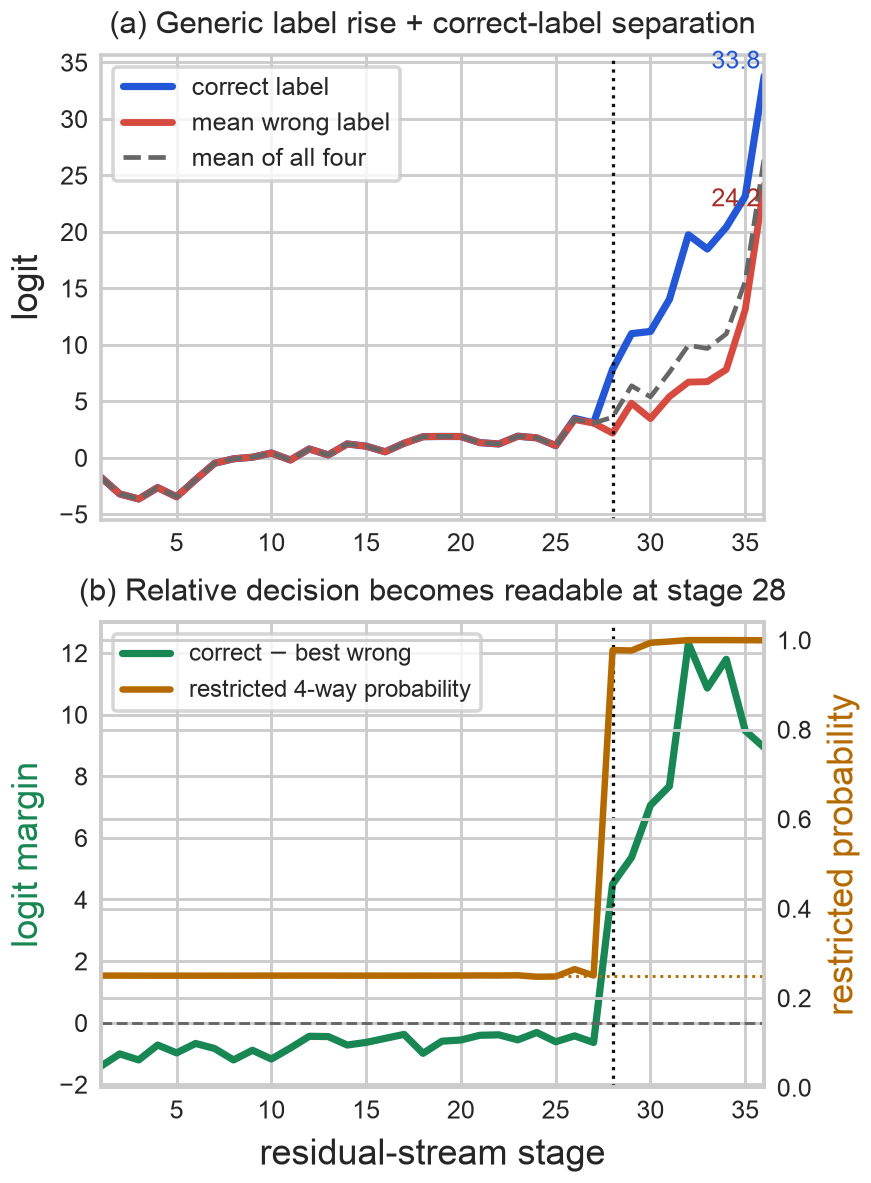
\includegraphics[width=\columnwidth]{figures/pilot_abcd_decomposition.png}
% \caption{All four familiar labels share a late rise, while the correct label
% separates on top of it. Stage 0 is omitted for readability. The logit lens is
% observational.}
% \label{fig:pilot-decomposition}
% \end{figure}

\begin{figure}[t]
    \centering
    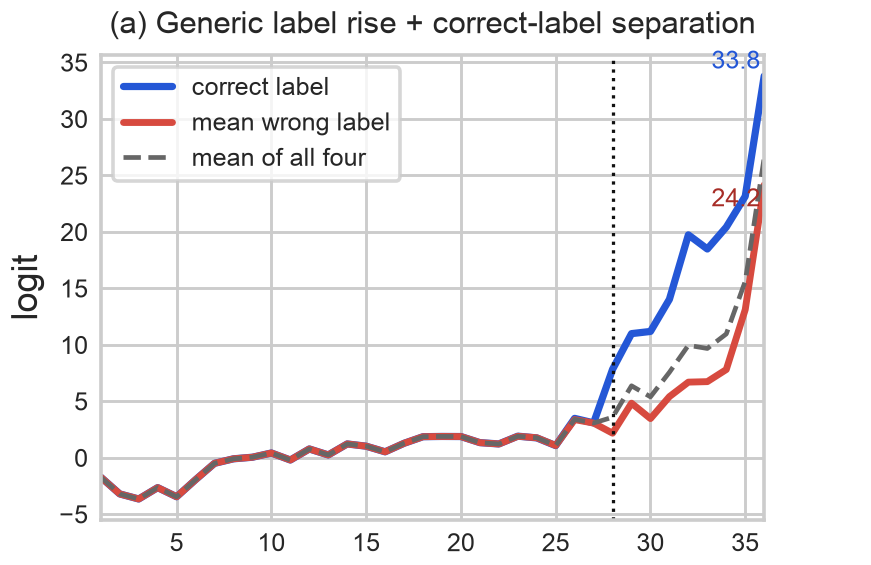
\includegraphics[width=0.48\columnwidth]{figures/pilot_abcd_decomposition_a.png}
    \hfill
    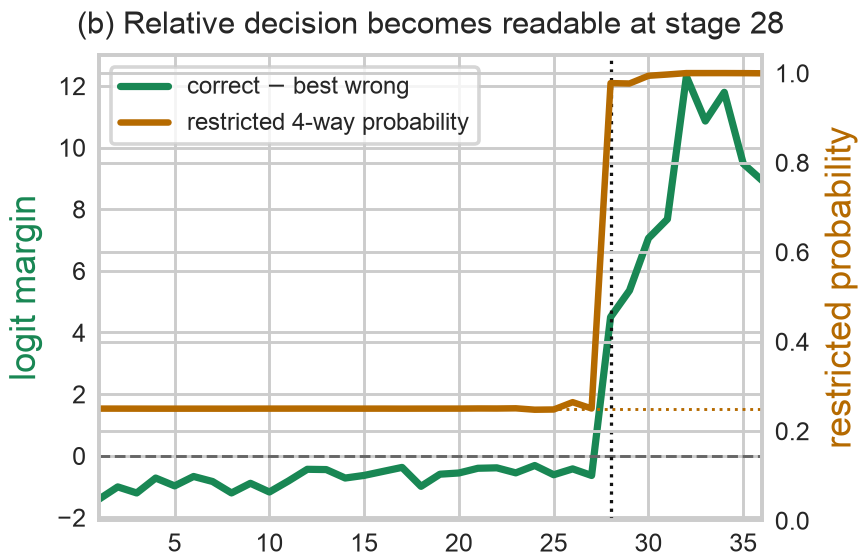
\includegraphics[width=0.48\columnwidth]{figures/pilot_abcd_decomposition_b.png}
    \caption{All four familiar labels share a late rise in the upper layers, while the correct label separates on top of it. Stage 0 being omitted for readability. The logit lens is observational.}
    \label{fig:pilot-decomposition}
\end{figure}

Correct-symbol separation is prior and strongest for A/B/C/D, later for
numbers, and latest and weakest for rare letters and punctuation. Q and !
account for all 42 unfamiliar-alphabet forced-choice errors, whereas A and 1
are perfect; the effect is therefore not a general first-position failure.
Default A/B/C/D directions can also dominate before the requested alphabet
takes over late.

\subsection{Causal pilot and working hypothesis}

Activation patching then tested whether a donor state could steer a recipient.
Table~\ref{tab:pilot-route} reports representative held-out effects. Normalized
recovery is 0 for no movement and 1 for full donor transfer.

% \begin{table*}[t]
% \centering
% \begin{tabularx}{\textwidth}{@{}lX@{}}
% \toprule
% Site & Representative result and supported reading \\
% \midrule
% Image, 0--16 & Recovery 0.92, 0.93, and 0.87: visual answer information is
% causally present early. \\
% Options, 20--25 & Content recovery peaks near 0.48: answer information later
% appears in candidate text. \\
% Labels, 26 & Position recovery is about 0.46: option identity associated
% with a displayed label. \\
% Final token, 27 & Symbol recovery is 0.76; attention 0.68 versus MLP 0.27, indicating a attention-mediated late update. \\
% Final token, 33 & Content recovery is 0.95; attention 0.55 versus MLP 0.03, while the answer becomes vocab-aligned. \\
% \bottomrule
% \end{tabularx}
% \caption{Representative causal pilot results. The sites support a sequence,
% not a proven edge-by-edge circuit.}
% \label{tab:pilot-route}
% \end{table*}

\begin{table}[t]
    \centering
    \begin{tabularx}{\columnwidth}{@{}lX@{}}
        \toprule
        Site & Representative result and supported reading \\
        \midrule
        Image, 0-16 & Recovery 0.92, 0.93, and 0.87: visual answer information is causally present early. \\

        Options, 20-25 & Content recovery peaks near 0.48: answer information later appears in candidate text. \\

        Labels, 26 & Position recovery is about 0.46: option identity associated with a displayed label. \\

        Final token, 27 & Symbol recovery is 0.76; attention 0.68 versus MLP 0.27, indicating an attention-mediated late update. \\

        Final token, 33 & Content recovery is 0.95; attention 0.55 versus MLP 0.03, while the answer becomes vocab-aligned. \\
        \bottomrule
    \end{tabularx}
    \caption{Representative causal pilot results. The sites support a sequence, not a proven edge-by-edge circuit.}
    \label{tab:pilot-route}
\end{table}

The pilot shows a testable route: visual content early, candidate states in
the middle, and a late position-to-symbol write. Image and option patches too
show why late vocabulary readability must not be mistaken for the
presence of answer information.

\section{Dataset and Model Selection}

\subsection{CLEVR-MCQ-4}

The proposal considered MMMU, a heterogeneous benchmark of expert-level
multimodal questions \citep{yue2024mmmu}. For repeatedly patched sub-10B
models, moderate baseline accuracy makes a failed intervention ambiguous. We
therefore built CLEVR-MCQ-4 from CLEVR's diagnostic scenes and
functional reasoning structure \citep{johnson2017clevr}.

The release covers nine reasoning families with type-matched distractors. It
contains three answer alphabets and five causal contrast types: position-only,
content-only, content-and-position, identity, and unrelated random pairs.
Splits are scene-disjoint and fixed before analysis (Table~\ref{tab:data}).
Figure~\ref{fig:clevr-example} illustrates the intended decomposition.

\begin{figure}[t]
\centering
\includegraphics[width=\columnwidth]{../../presentation/assets/e06_pair_000012_x.png}
\caption{Example task: identify the brown object through a visual relation,
locate ``brown'' among the options, and emit its assigned label A.}
\label{fig:clevr-example}
\end{figure}

\begin{table}[t]
\centering
\begin{tabularx}{\columnwidth}{l r X}
\toprule
Split & Items & Use \\
\midrule
Calibration & 120 & Dataset checks only \\
Screening & 300 & Optional model screen \\
Behaviour & 256 & Accuracy and lenses \\
Discovery & 320 & Select layers and heads \\
Confirmation & 256 & Frozen held-out tests \\
\midrule
Total & 1,252 & 17,328 prompt variants \\
\bottomrule
\end{tabularx}
\caption{Frozen CLEVR-MCQ-4 release. Discovery has 160 pairs and confirmation
has 128 pairs.}
\label{tab:data}
\end{table}

\begin{table*}[t]
\centering
\begin{tabularx}{\textwidth}{@{}l>{\raggedright\arraybackslash}Xrrr@{\hspace{1em}}l>{\raggedright\arraybackslash}Xrrr@{}}
\toprule
Family & Model (B) & Acc. & Gap & D/C & Family & Model (B) & Acc. & Gap & D/C \\
\midrule
Qwen & Qwen2-VL (2.2) & .7292 & .4167 & 6/4 & LLaVA-OV & 0.5B-SI (0.9) & .4063 & .1771 & 1/2 \\
Qwen & Qwen2.5-VL (3.8) & .8438 & .5729 & 6/6 & LLaVA-OV & \textbf{7B-SI (8.0)} & \textbf{.7292} & \textbf{.4479} & \textbf{3/4} \\
Qwen & \textbf{Qwen2.5-VL (8.3)} & \textbf{.9375} & \textbf{.6458} & \textbf{6/6} & LLaVA-OV & 7B-OV (8.0) & .6458 & .3542 & 6/6 \\
InternVL & 3.5-1B (1.1) & .8750 & .5417 & 5/4 & PaliGemma & 3B Mix (2.9) & .4271 & .2292 & 4/3 \\
InternVL & 3.5-2B (2.3) & .9063 & .6667 & 4/5 & PaliGemma & 2-3B Mix (3.0) & .5000 & .2604 & 2/3 \\
InternVL & \textbf{3.5-8B (8.5)} & \textbf{1.0000} & \textbf{.7813} & \textbf{6/5} & PaliGemma & \textbf{2-10B Mix (9.7)} & \textbf{.5833} & \textbf{.3958} & \textbf{2/3} \\
\bottomrule
\end{tabularx}
\caption{Condensed 24-item model screen. Accuracy is restricted A/B/C/D
accuracy; Gap is clean minus shuffled-image accuracy; D/C gives available
discovery/confirmation pairs. Worst-position accuracy was also checked. Bold
marks the provisional family representative.}
\label{tab:screen}
\end{table*}


\subsection{Model screening}

The same 24-item smoke profile tested three checkpoints from each of four
families: Qwen, InternVL, LLaVA-OneVision, and PaliGemma
\citep{bai2025qwen25vl,wang2025internvl35,li2024llavaov,beyer2024paligemma}.
The screen checked adapter and intervention compatibility, task performance,
image dependence, and available causal pairs. It guides selection rather than
serving as a leaderboard because each estimate uses only 24 items.

Qwen2.5-VL-7B and InternVL3.5-8B offered the strongest combination of
image-dependent performance, calibrated interventions, sufficient pairs, and
feasible size. The 24-item estimates remain screening evidence and are not
pooled with the causal runs.

The sequential full InternVL discovery-to-confirmation sweep was projected
from measured throughput to require roughly 50--60 hours. To obtain a timely
cross-model test without reducing layer resolution or interrupting that run,
we used a separate report track with 32 pair-balanced counterfactual cases per
contrast in each disjoint split, rather than 64. It retained the same frozen
release, checkpoint, prompts, gates, hooks, all 36 residual layers, and
discovery-before-confirmation protocol; its estimates are therefore a smaller
matched replication, reported as preliminary until the full sweep is audited.

\section{Core-7 Methodology}

Core-7 combines four interventions with three descriptive readouts. For donor
and recipient examples, normalized recovery is
$\nr=(s_{\mathrm{patched}}-s_{\mathrm{recipient}})/
(s_{\mathrm{donor}}-s_{\mathrm{recipient}})$ for a predeclared logit
difference $s$. We also report flip rate, the fraction of patched predictions
that become the donor answer. Recovery can change without a categorical flip.

\begin{table*}[t]
\centering
\begin{tabularx}{\textwidth}{@{}l p{0.27\textwidth} X@{}}
\toprule
 & Plain-language question & Measurement and evidential role \\
\midrule
\method{1} & When can a donor answer steer the output? & Patch the final-token
state by layer; random pairs test whether transfer is contrast-specific. \\
\method{2} & Does attention or the MLP matter more? & Patch and ablate their
updates separately; vocabulary projections remain descriptive. \\
\method{3} & Do a few attention heads dominate? & Select heads on discovery,
freeze them, and compare with layer-matched random sets on confirmation. \\
\method{4} & When is the answer label readable? & Project every residual stage
to the vocabulary; this measures accessibility, not causal origin. \\
\method{5} & Is content readable before the symbol? & Compare answer-word and
answer-label projections through depth. \\
\method{6} & Which token groups carry the effect? & Patch image, question,
option, label, and final-token groups under controlled contrasts. \\
\method{7} & Do unfamiliar labels change the route? & Repeat behaviour and
readouts across alphabets, including default A/B/C/D directions. \\
\bottomrule
\end{tabularx}
\caption{Core-7. M1, M2, M3, and M6 intervene on activations. M4, M5, and M7
are observational readouts and are interpreted accordingly.}
\label{tab:core7}
\end{table*}

All selection decisions use discovery data and are frozen before confirmation.
The full Qwen workflow uses 64 pairs and 28 decoder layers. The preliminary
InternVL track uses 32 pair-balanced cases per contrast and all 36 layers;
token groups are sampled every second layer, and frozen head sets are compared
with ten exact-size, layer-matched random sets. Reported sample sizes remain
attached to their experiments; smoke, preliminary, and full results are not
pooled.

\section{Results}

\subsection{Behavioural foundation}

The 256-item Qwen behavioural set establishes that the model solves the task
using visual evidence. Accuracy is 83.7\% with A/B/C/D, 80.3\% with numbers, and
82.2\% with rare letters. It falls to 28.5\% with a blank image and 29.6\%
with a shuffled image (Figure~\ref{fig:qwen-behaviour}). Logical OR remains
difficult at 44.7\%, so subsequent causal averages use pairs for which donor
and recipient are both answered correctly. On the matched 24-item screen,
InternVL reaches 100.0\% A/B/C/D accuracy and loses 78.1 percentage points
when images are shuffled. This smaller estimate establishes feasibility and
image dependence; it is not pooled with Qwen's 256-item result.

% \begin{figure*}[t]
% \centering
% 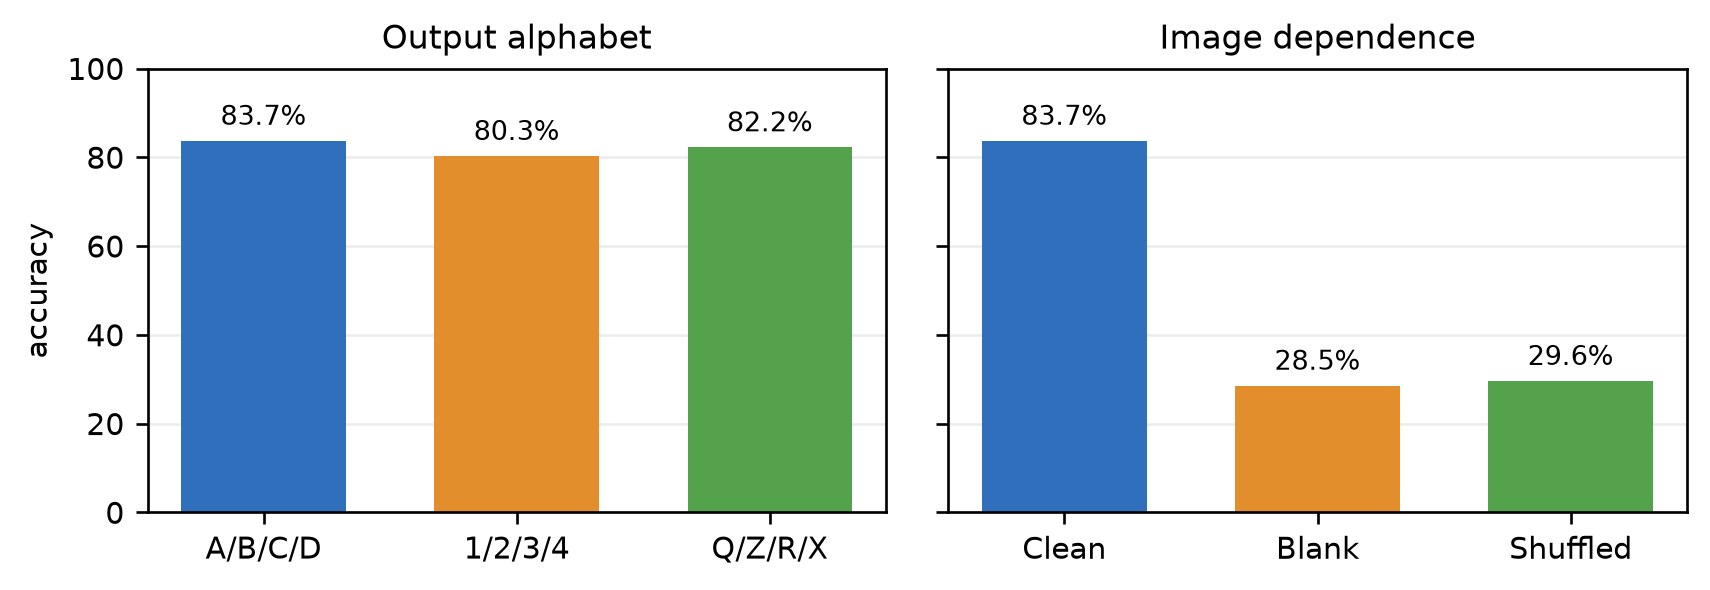
\includegraphics[width=0.72\textwidth]{figures/qwen_behavior_controls.png}
% \caption{Accuracy is similar across output alphabets but collapses when useful
% visual evidence is removed or mismatched.}
% \label{fig:qwen-behaviour}
% \end{figure*}

\begin{figure}[t]
    \centering
    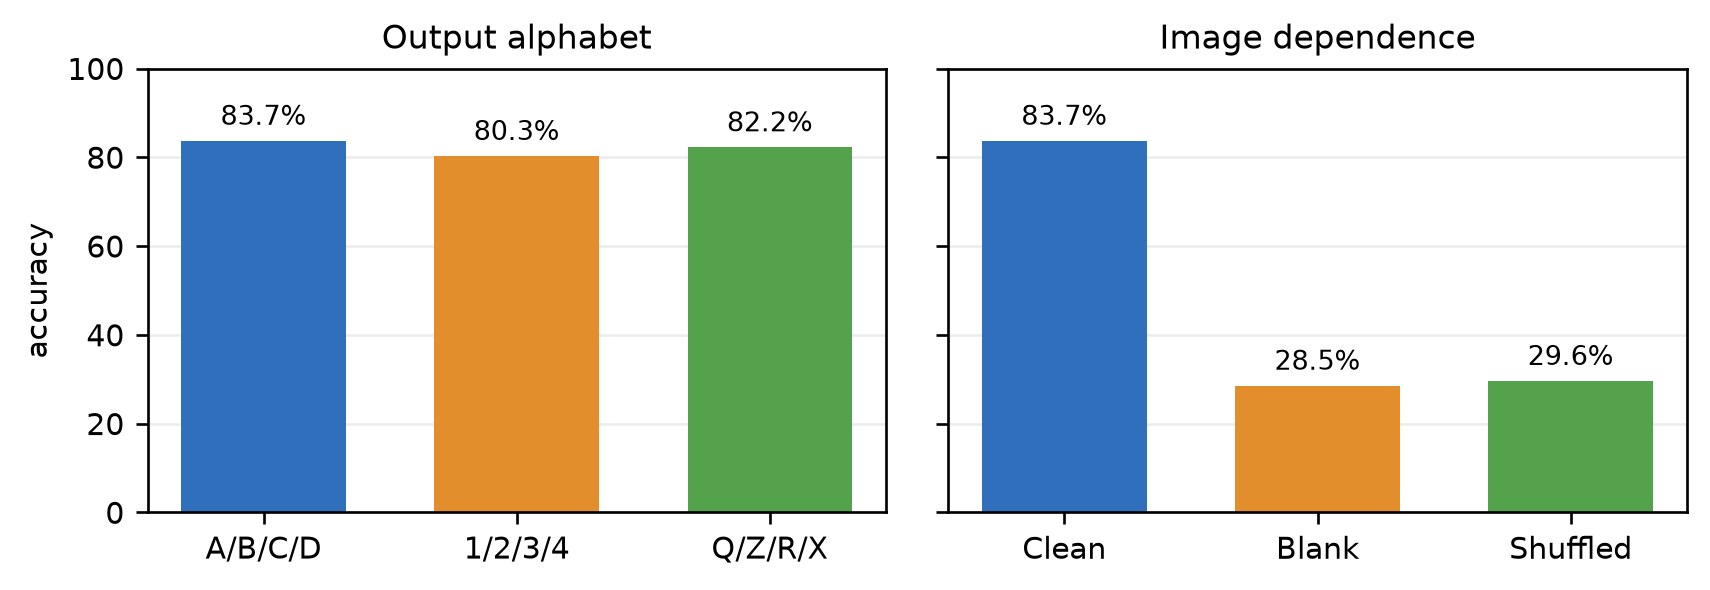
\includegraphics[width=\columnwidth]{figures/qwen_behavior_controls.png}
    \caption{Accuracy is similar across output alphabets but collapses when useful visual evidence is removed or mismatched.}
    \label{fig:qwen-behaviour}
\end{figure}

\subsection{M1 and M6: when and where the answer transfers}

\paragraph{Method.}
M1 patches the final answer-token state from a donor into a recipient at each
layer. M6 instead patches token groups to identify the carrier of the effect.

\paragraph{Results.}
M1's final-token transfer crosses its frozen threshold at layer 24 on both
discovery and confirmation. For position-only pairs, the donor-label flip rate
rises from 2.7\% at layer 23 to 73.5\% at 24, 84.9\% at 25, and 100.0\% by
27. However, unrelated random pairs transfer almost as strongly
(Figure~\ref{fig:compare-m1m6}). M1 therefore establishes a late transferable donor
state, but does not by itself isolate a contrast-specific binding code.

M6 supplies the carrier information. Under content contrasts, image-token
recovery is 101.0\% through layers 0-8, falls to 24.0\% at layer 16 and 6.0\%
at layer 24, while option-content recovery reaches 38.0\% at layer 16 and peaks
at 43.0\% at layer 18. In content-and-position confirmation pairs, final-token
patches primarily transfer the donor position/symbol: position flips rise from
74.0\% at layer 24 to 100.0\% at 27. Together, M1 and M6 support an early
image-token carrier, a middle option-content carrier, and a late output-symbol
state.

InternVL reproduces this ordering on its disjoint confirmation split:
position transfer crosses threshold at layer 29 and content transfer at 31.
At layer 29, position recovery is 54.2\% and the donor-position flip rate is
71.9\%. Its random-pair recovery is again stronger (68.3\%), so the same
interpretive restriction applies. M6 also begins with strong image-token
recovery and peaks later in question and option-content tokens. The shared
result is an image-to-text-to-symbol route; Qwen's late transition is sharper,
whereas InternVL's develops more gradually.

\begin{figure*}[t]
\centering
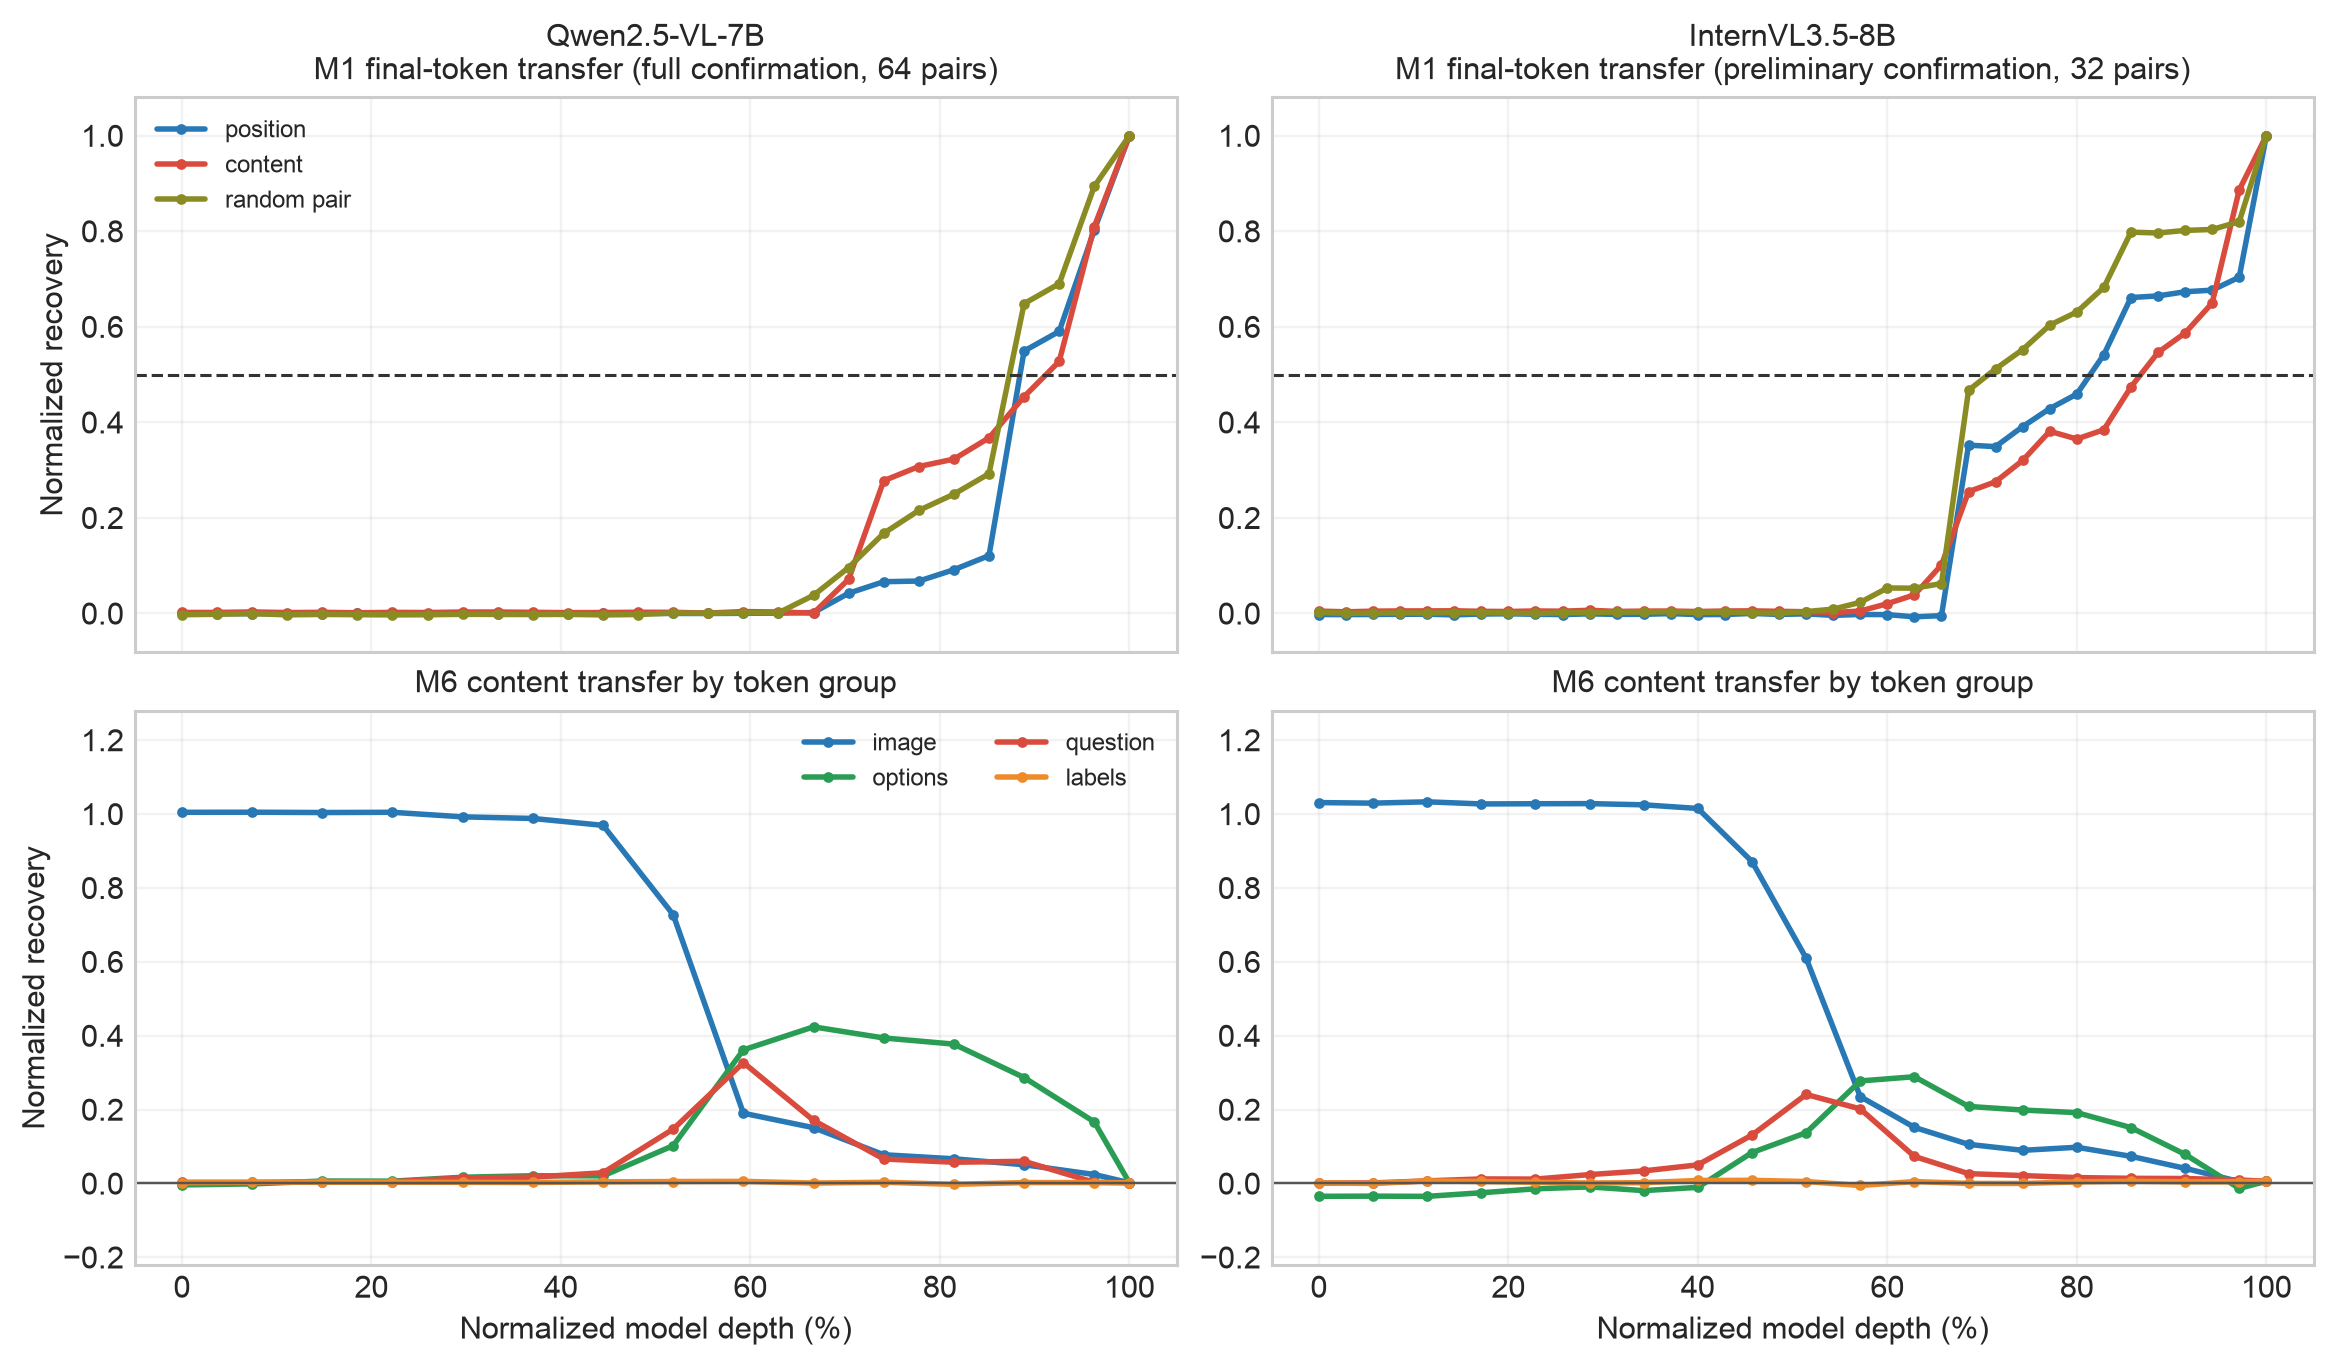
\includegraphics[width=0.92\textwidth]{figures/compare_m1_m6.png}
\caption{M1 and M6 on held-out pairs. Top: final-token recovery for position,
content, and random donors. Bottom: content recovery by patched token group.
Depth is normalized across Qwen's 28 layers (64 pairs) and InternVL's 36
layers (32 preliminary pairs).}
\label{fig:compare-m1m6}
\end{figure*}

\subsection{M2: attention and MLP contributions}

\paragraph{Method.}
M2 patches and resampling-ablates the attention and MLP updates separately. A
direct vocabulary projection is included only to describe what each update
aligns with.

\paragraph{Results.}
Attention-output patch recovery peaks at layer 24: 44.1\% on discovery and
43.9\% on confirmation, versus an MLP peak near 10.0\%. Resampling the layer-24
attention update reduces the correct-label margin by 5.0 logits, compared with
0.6 for the MLP. At the final layer, MLP ablation has the larger effect (1.5
versus 0.7 logits). The projection in Figure~\ref{fig:qwen-m2} shows a sharp
layer-24 attention write to the correct-minus-wrong margin, whereas late MLP
updates align more with a shared rise in candidate-label logits. The causal
evidence comes from patching and ablation, not from the projection alone.

InternVL shows the same component division. Confirmation attention recovery
peaks at 35.0\% at layer 24, compared with a 4.6\% MLP peak; resampling the
layer-24 attention update reduces the answer margin by 5.1 logits, while the
MLP change is $-0.1$. Thus the main discriminative write is
attention-mediated in both models, while the projection-based generic-label
interpretation remains descriptive.

\begin{figure*}[t]
\centering
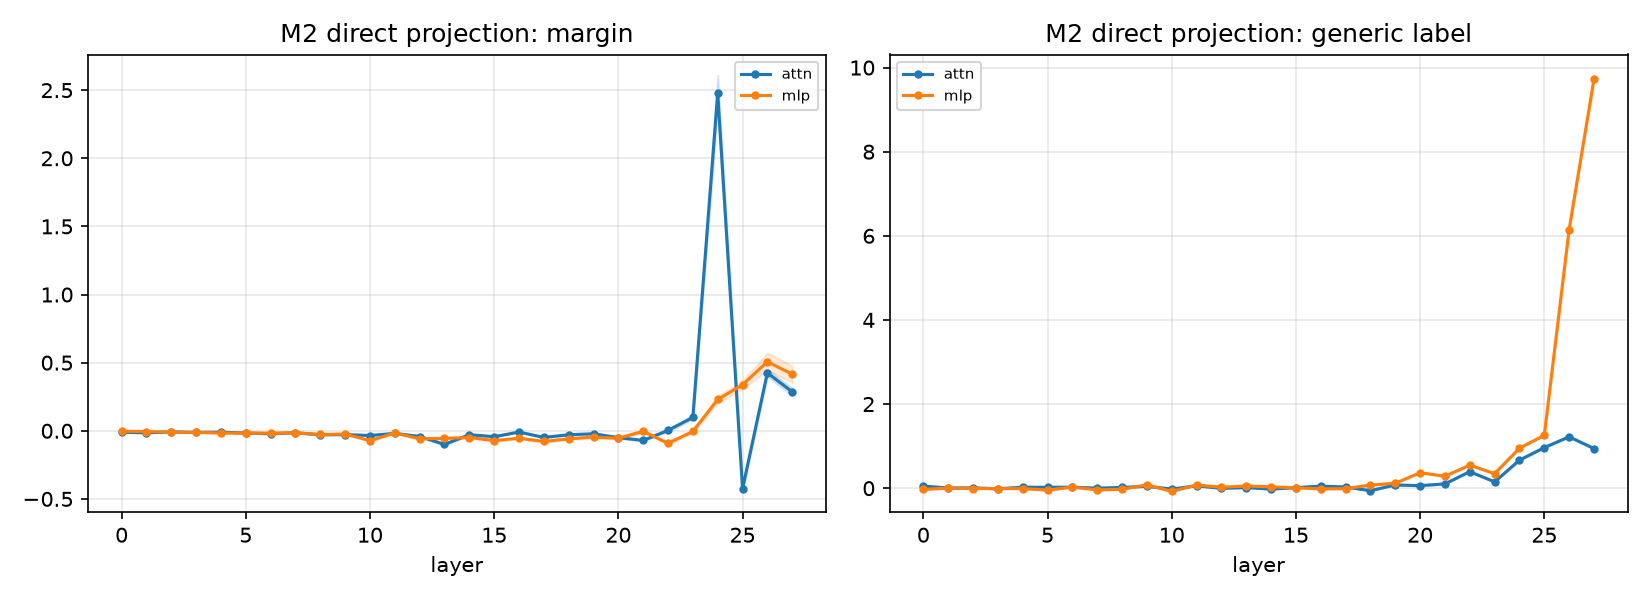
\includegraphics[width=0.78\textwidth]{figures/qwen_m2_projection.png}
\caption{M2 direct projection. Attention has its
largest discriminative write near layer 24 (left); late MLP updates show the
largest generic candidate-label write (right).}
\label{fig:qwen-m2}
\end{figure*}

\subsection{M3: important heads, with model-dependent sparsity}

\paragraph{Method.}
M3 ranks heads with equal pair weight, freezes each top-$k$ set, and evaluates
it on a disjoint confirmation split. Qwen uses 64 pairs per split and InternVL
uses 32; exact-size, layer-matched random sets form each null distribution.

\par\noindent\textbf{Results.}\quad
Confirmation recovery rises from 11.6\% for one head to 24.4\% for two, 41.7\%
for four, 68.4\% for eight, and 89.5\% for sixteen. Four heads recover 52.7\%
of the all-head reference and exceed the matched-random 95th percentile of
6.9\%, satisfying the predeclared sparse-set criterion
(Figure~\ref{fig:qwen-m3}). This establishes a reproducible, concentrated
causal effect, not a complete or uniquely necessary circuit.

InternVL's frozen sets also have a clear held-out effect: one, four, and
sixteen heads recover 20.4\%, 43.1\%, and 92.4\%, and every tested top-$k$
set exceeds its matched-random 95th percentile. The sparsity classification is
not stable, however. Four heads recover 49.9\% of the all-head effect in
discovery but 50.8\% in confirmation. The predeclared verdict therefore moves
from ``distributed'' to ``sparse'' at its 50\% boundary. We infer selected head
concentration in both models, but stable sparsity only in Qwen.

\begin{figure*}[t]
\centering
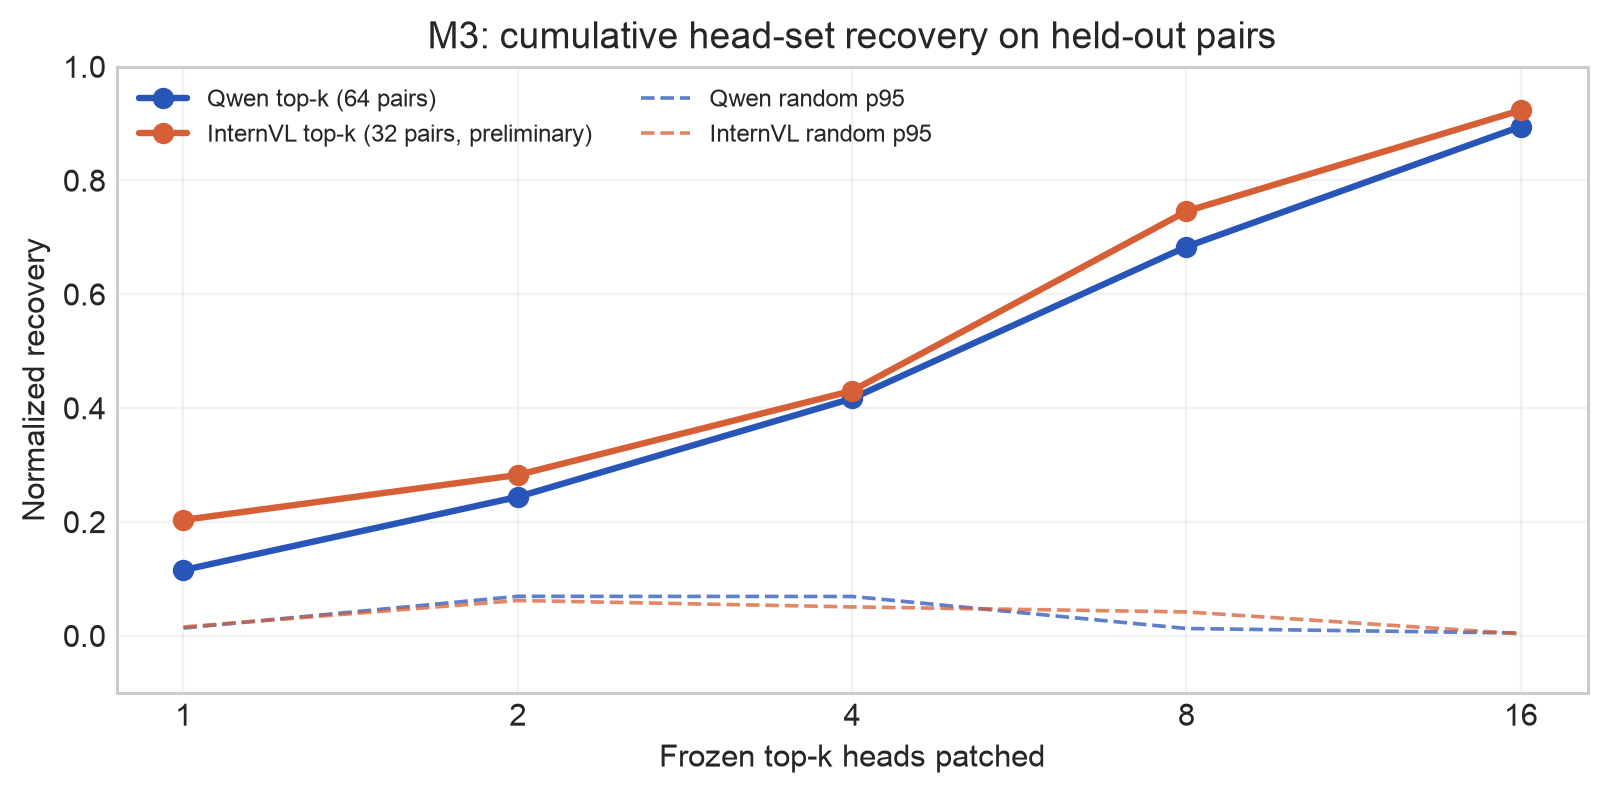
\includegraphics[width=0.62\textwidth]{figures/compare_m3.png}
\caption{M3 confirmation recovery for frozen top-$k$ head sets. Dashed curves
show layer-matched random 95th percentiles. InternVL's selected-head effect is
clear, but its sparse/distributed verdict does not replicate.}
\label{fig:qwen-m3}
\end{figure*}

\subsection{M4, M5, and M7: readable content and output symbols}

\paragraph{Method.}
M4 follows the answer labels through depth, M5 compares the semantic answer
word with the printed label, and M7 repeats the readout for different output
alphabets. All three are vocabulary projections: they measure linear
readability in the final vocabulary basis, not causal use.

\paragraph{Results.}
The familiar-letter margin becomes stably positive around stages 22-23 of 28;
numbers follow at 23 and rare letters at 24. All candidate labels also receive
a shared late lift (Figure~\ref{fig:qwen-m4m7}). For rare-label prompts, the
requested alphabet holds only 12.6\% of the combined requested/default
eight-way mass at stage 24, then 82.8\% at 25. The final-token answer word does
not become stably positive until stage 27, after the answer symbol is already
readable (Figure~\ref{fig:qwen-m5}). M6 prevents this late content-word readout
from being mistaken for the first presence of answer content: content has
earlier causal carriers in image and option tokens.

The available matched InternVL lens evidence is the six-pair smoke analysis,
not the 32-pair causal track. It nevertheless gives the same qualitative
ordering: A-D labels become stably readable at stage 25 of 36, the requested
rare alphabet overtakes default A-D directions at stage 30, and the content
word becomes readable at stage 32. Across models, output-symbol alignment
therefore precedes final-token content-word alignment, while M6 shows that
answer content is causally active at earlier non-final token sites.

\begin{figure*}[t]
\centering
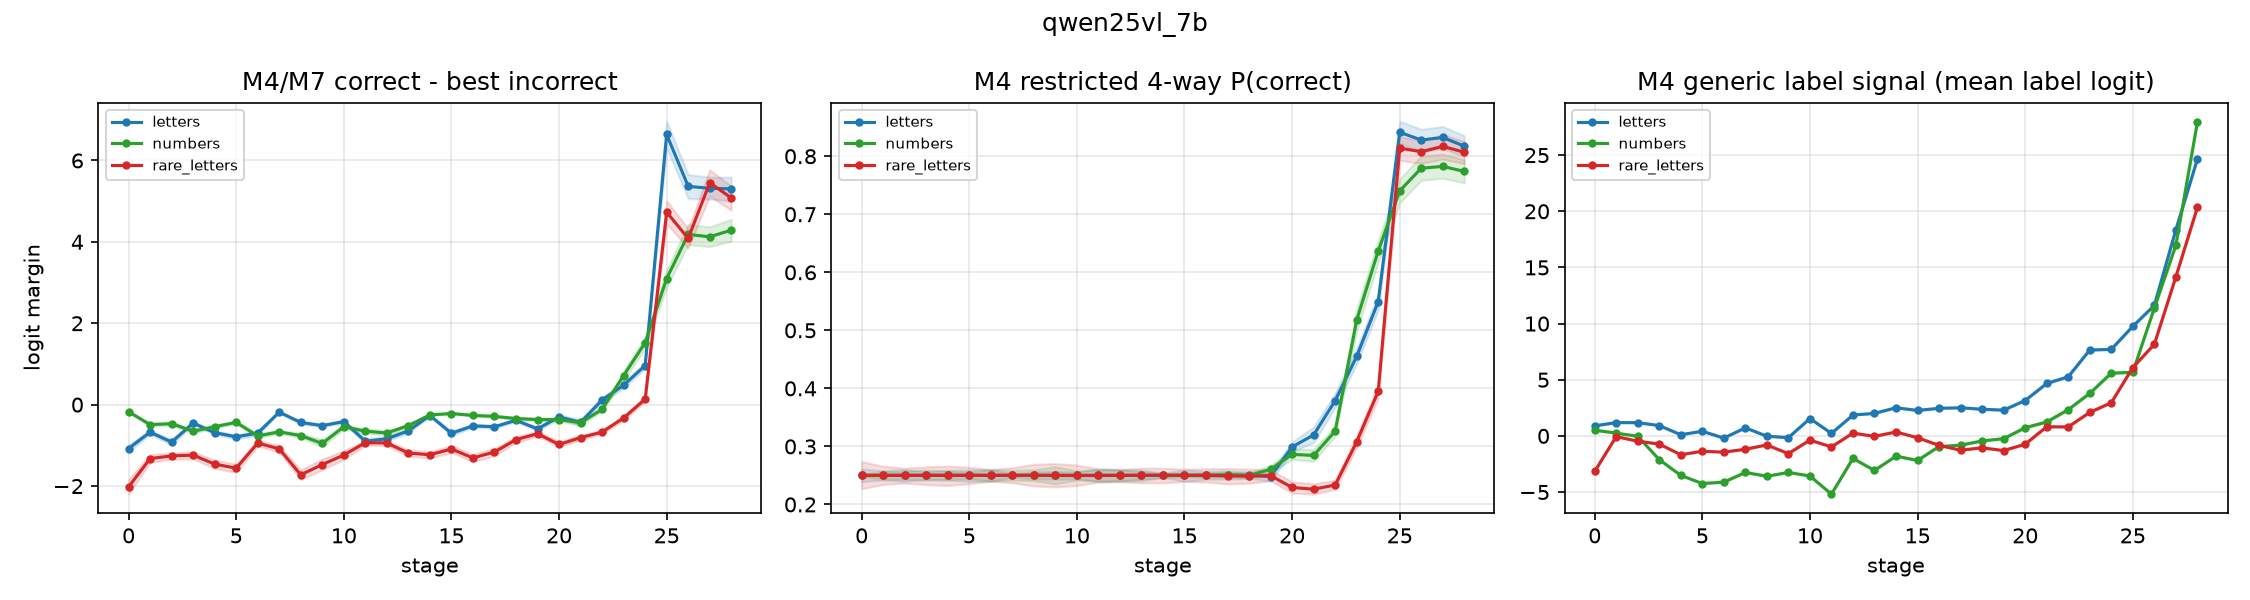
\includegraphics[width=0.78\textwidth]{figures/qwen_m4_m7_lens.png}
\caption{M4/M7 readouts. Correct-label separation,
restricted confidence, and the shared candidate-label lift all emerge late.}
\label{fig:qwen-m4m7}
\end{figure*}

\begin{figure*}[t]
\centering
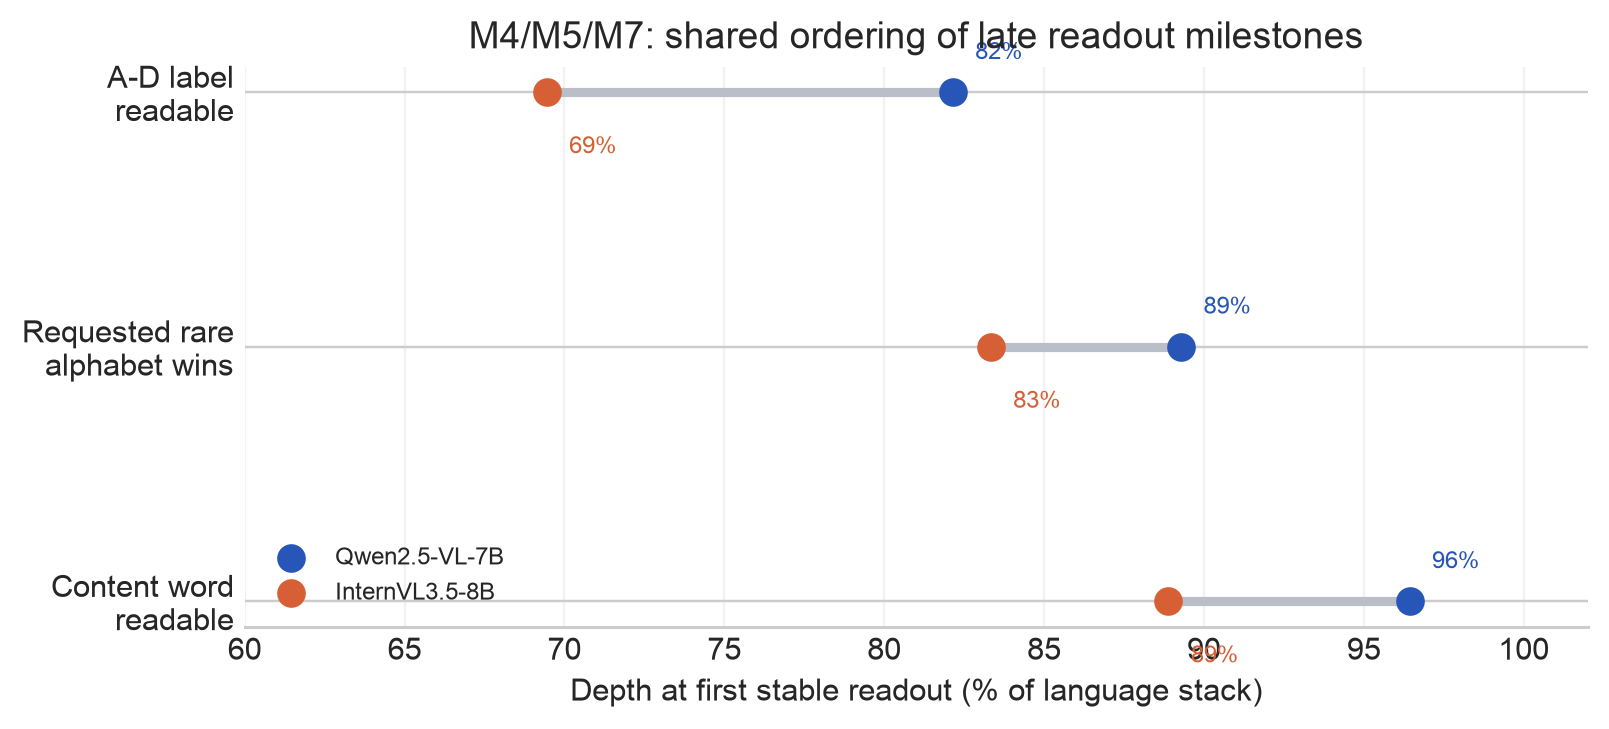
\includegraphics[width=0.58\textwidth]{figures/compare_lens_milestones.png}
\caption{Matched M4/M5/M7 readout milestones, normalized by language-stack
depth. InternVL milestones come from the six-pair smoke lens and remain
preliminary. The shared result is the ordering, not identical absolute depth.}
\label{fig:qwen-m5}
\end{figure*}

\section{Cross-model Interpretation}

Both models support the same broad computation: visual states carry answer
content early, textual option states become useful in the middle, and late
attention has the largest causal effect on the emitted position/symbol. They
also share strong random-pair portability and a late switch from default
A/B/C/D directions into the requested output alphabet. The main differences
are quantitative: InternVL's late transfer is more gradual, and its sparse-head
verdict is threshold-sensitive at 32 pairs. Agreement therefore strengthens
the staged VLM-level account, while the unstable head result identifies the
claim most in need of the continuing full InternVL sweep.

\section{Conclusion}

Qwen and preliminary InternVL evidence support a staged account:
answer-relevant information is causally present in image tokens early,
textual option states become useful in the middle, and late attention strongly
affects the selected output symbol. Frozen head sets have substantial held-out
effects in both models, although only Qwen currently supports a stable sparse
verdict. Vocabulary projections reveal late label readability and alphabet
switching rather than the first computation of answer content. The account is
deliberately narrower than a complete circuit claim: strong random-pair
transfer shows that late donor-state portability is not specific to the
controlled semantic contrast.

\section*{Limitations}

The study covers two 8B-class VLMs on one controlled dataset, and both language
backbones are Qwen-lineage. InternVL causal estimates use 32 pair-balanced
cases per contrast and remain preliminary until the longer full sweep is
complete and audited. Some question families remain difficult, and causal
analyses condition on correct donor/recipient pairs. Patching supports effects
only for the tested source, target, site, and metric; vocabulary projections
remain correlational. Neither model's selected heads constitute a complete or
unique circuit.

\section{Timeline}

\begin{table}[ht]
\centering
\small
\begin{tabularx}{\columnwidth}{@{}l X@{}}
\toprule
\textbf{Dates} & \textbf{Milestone} \\ 
% \midrule

% Aug 28 -- Sep 7 
% & Set up all four models and build the question-variant generator. \\ 
% \addlinespace[0.5ex]

% Sep 8 -- Sep 21 
% & Screen models and select the best one per family; build the activation-patching pipeline; begin layer patching and logit-lens analysis. \\ 
% \addlinespace[0.5ex]

% Sep 22 -- Sep 30 
% & Complete layer patching, attention/MLP decomposition, and logit-lens analysis on at least two model families. \\

% \midrule
\multicolumn{2}{c}{\textit{Mid-submission: Octoberr 31st}} \\

\midrule

Oct 1 -- Oct 12 
& Complete the remaining core experiments across all four model families. \\ 
\addlinespace[0.5ex]

Oct 13 -- Oct 24 
& Conduct stretch experiments, prioritizing cross-image patching and failure-mode analysis, followed by remaining experiments if time permits. \\ 
\addlinespace[0.5ex]

Oct 25 -- Oct 31 
& Consolidate results, prepare figures, and write the final report. \\

\midrule
\multicolumn{2}{c}{\textit{Final submission: October 31}} \\

\bottomrule
\end{tabularx}
\caption{Project Timeline}
\label{tab:timeline}
\end{table}


% \section{Engines}

% To produce a PDF file, pdf\LaTeX{} is strongly recommended (over original \LaTeX{} plus dvips+ps2pdf or dvipdf).
% The style file \texttt{acl.sty} can also be used with
% lua\LaTeX{} and
% Xe\LaTeX{}, which are especially suitable for text in non-Latin scripts.
% The file \texttt{acl\_lualatex.tex} in this repository provides
% an example of how to use \texttt{acl.sty} with either
% lua\LaTeX{} or
% Xe\LaTeX{}.

% \section{Preamble}

% The first line of the file must be
% \begin{quote}
% \begin{verbatim}
% \documentclass[11pt]{article}
% \end{verbatim}
% \end{quote}

% To load the style file in the review version:
% \begin{quote}
% \begin{verbatim}
% \usepackage[review]{acl}
% \end{verbatim}
% \end{quote}
% For the final version, omit the \verb|review| option:
% \begin{quote}
% \begin{verbatim}
% \usepackage{acl}
% \end{verbatim}
% \end{quote}

% To use Times Roman, put the following in the preamble:
% \begin{quote}
% \begin{verbatim}
% \usepackage{times}
% \end{verbatim}
% \end{quote}
% (Alternatives like txfonts or newtx are also acceptable.)

% Please see the \LaTeX{} source of this document for comments on other packages that may be useful.

% Set the title and author using \verb|\title| and \verb|\author|. Within the author list, format multiple authors using \verb|\and| and \verb|\And| and \verb|\AND|; please see the \LaTeX{} source for examples.

% By default, the box containing the title and author names is set to the minimum of 5 cm. If you need more space, include the following in the preamble:
% \begin{quote}
% \begin{verbatim}
% \setlength\titlebox{<dim>}
% \end{verbatim}
% \end{quote}
% where \verb|<dim>| is replaced with a length. Do not set this length smaller than 5 cm.

% \section{Document Body}

% \subsection{Footnotes}

% Footnotes are inserted with the \verb|\footnote| command.\footnote{This is a footnote.}

% \subsection{Tables and figures}

% See Table~\ref{tab:accents} for an example of a table and its caption.
% \textbf{Do not override the default caption sizes.}

% \begin{table}
%   \centering
%   \begin{tabular}{lc}
%     \hline
%     \textbf{Command} & \textbf{Output} \\
%     \hline
%     \verb|{\"a}|     & {\"a}           \\
%     \verb|{\^e}|     & {\^e}           \\
%     \verb|{\`i}|     & {\`i}           \\
%     \verb|{\.I}|     & {\.I}           \\
%     \verb|{\o}|      & {\o}            \\
%     \verb|{\'u}|     & {\'u}           \\
%     \verb|{\aa}|     & {\aa}           \\\hline
%   \end{tabular}
%   \begin{tabular}{lc}
%     \hline
%     \textbf{Command} & \textbf{Output} \\
%     \hline
%     \verb|{\c c}|    & {\c c}          \\
%     \verb|{\u g}|    & {\u g}          \\
%     \verb|{\l}|      & {\l}            \\
%     \verb|{\~n}|     & {\~n}           \\
%     \verb|{\H o}|    & {\H o}          \\
%     \verb|{\v r}|    & {\v r}          \\
%     \verb|{\ss}|     & {\ss}           \\
%     \hline
%   \end{tabular}
%   \caption{Example commands for accented characters, to be used in, \emph{e.g.}, Bib\TeX{} entries.}
%   \label{tab:accents}
% \end{table}

% As much as possible, fonts in figures should conform
% to the document fonts. See Figure~\ref{fig:experiments} for an example of a figure and its caption.

% Using the \verb|graphicx| package graphics files can be included within figure
% environment at an appropriate point within the text.
% The \verb|graphicx| package supports various optional arguments to control the
% appearance of the figure.
% You must include it explicitly in the \LaTeX{} preamble (after the
% \verb|\documentclass| declaration and before \verb|\begin{document}|) using
% \verb|\usepackage{graphicx}|.

% \begin{figure}[t]
%   \includegraphics[width=\columnwidth]{example-image-golden}
%   \caption{A figure with a caption that runs for more than one line.
%     Example image is usually available through the \texttt{mwe} package
%     without even mentioning it in the preamble.}
%   \label{fig:experiments}
% \end{figure}

% \begin{figure*}[t]
%   \includegraphics[width=0.48\linewidth]{example-image-a} \hfill
%   \includegraphics[width=0.48\linewidth]{example-image-b}
%   \caption {A minimal working example to demonstrate how to place
%     two images side-by-side.}
% \end{figure*}

% \subsection{Hyperlinks}

% Users of older versions of \LaTeX{} may encounter the following error during compilation:
% \begin{quote}
% \verb|\pdfendlink| ended up in different nesting level than \verb|\pdfstartlink|.
% \end{quote}
% This happens when pdf\LaTeX{} is used and a citation splits across a page boundary. The best way to fix this is to upgrade \LaTeX{} to 2018-12-01 or later.

% \subsection{Citations}

% \begin{table*}
%   \centering
%   \begin{tabular}{lll}
%     \hline
%     \textbf{Output}           & \textbf{natbib command} & \textbf{ACL only command} \\
%     \hline
%     \citep{Gusfield:97}       & \verb|\citep|           &                           \\
%     \citealp{Gusfield:97}     & \verb|\citealp|         &                           \\
%     \citet{Gusfield:97}       & \verb|\citet|           &                           \\
%     \citeyearpar{Gusfield:97} & \verb|\citeyearpar|     &                           \\
%     \citeposs{Gusfield:97}    &                         & \verb|\citeposs|          \\
%     \hline
%   \end{tabular}
%   \caption{\label{citation-guide}
%     Citation commands supported by the style file.
%     The style is based on the natbib package and supports all natbib citation commands.
%     It also supports commands defined in previous ACL style files for compatibility.
%   }
% \end{table*}

% Table~\ref{citation-guide} shows the syntax supported by the style files.
% We encourage you to use the natbib styles.
% You can use the command \verb|\citet| (cite in text) to get ``author (year)'' citations, like this citation to a paper by \citet{Gusfield:97}.
% You can use the command \verb|\citep| (cite in parentheses) to get ``(author, year)'' citations \citep{Gusfield:97}.
% You can use the command \verb|\citealp| (alternative cite without parentheses) to get ``author, year'' citations, which is useful for using citations within parentheses (e.g. \citealp{Gusfield:97}).

% A possessive citation can be made with the command \verb|\citeposs|.
% This is not a standard natbib command, so it is generally not compatible
% with other style files.

% \subsection{References}

% \nocite{Ando2005,andrew2007scalable,rasooli-tetrault-2015}

% The \LaTeX{} and Bib\TeX{} style files provided roughly follow the American Psychological Association format.
% If your own bib file is named \texttt{custom.bib}, then placing the following before any appendices in your \LaTeX{} file will generate the references section for you:
% \begin{quote}
% \begin{verbatim}
% \bibliography{custom}
% \end{verbatim}
% \end{quote}

% You can obtain the complete ACL Anthology as a Bib\TeX{} file from \url{https://aclweb.org/anthology/anthology.bib.gz}.
% To include both the Anthology and your own .bib file, use the following instead of the above.
% \begin{quote}
% \begin{verbatim}
% \bibliography{anthology,custom}
% \end{verbatim}
% \end{quote}

% Please see Section~\ref{sec:bibtex} for information on preparing Bib\TeX{} files.

% \subsection{Equations}

% An example equation is shown below:
% \begin{equation}
%   \label{eq:example}
%   A = \pi r^2
% \end{equation}

% Labels for equation numbers, sections, subsections, figures and tables
% are all defined with the \verb|\label{label}| command and cross references
% to them are made with the \verb|\ref{label}| command.

% This an example cross-reference to Equation~\ref{eq:example}.

% \subsection{Appendices}

% Use \verb|\appendix| before any appendix section to switch the section numbering over to letters. See Appendix~\ref{sec:appendix} for an example.

% \section{Bib\TeX{} Files}
% \label{sec:bibtex}

% Unicode cannot be used in Bib\TeX{} entries, and some ways of typing special characters can disrupt Bib\TeX's alphabetization. The recommended way of typing special characters is shown in Table~\ref{tab:accents}.

% Please ensure that Bib\TeX{} records contain DOIs or URLs when possible, and for all the ACL materials that you reference.
% Use the \verb|doi| field for DOIs and the \verb|url| field for URLs.
% If a Bib\TeX{} entry has a URL or DOI field, the paper title in the references section will appear as a hyperlink to the paper, using the hyperref \LaTeX{} package.

% \section*{Limitations}

% This document does not cover the content requirements for ACL or any
% other specific venue.  Check the author instructions for
% information on
% maximum page lengths, the required ``Limitations'' section,
% and so on.

% \section*{Acknowledgments}

% This document has been adapted
% by Steven Bethard, Ryan Cotterell and Rui Yan
% from the instructions for earlier ACL and NAACL proceedings, including those for
% ACL 2019 by Douwe Kiela and Ivan Vuli\'{c},
% NAACL 2019 by Stephanie Lukin and Alla Roskovskaya,
% ACL 2018 by Shay Cohen, Kevin Gimpel, and Wei Lu,
% NAACL 2018 by Margaret Mitchell and Stephanie Lukin,
% Bib\TeX{} suggestions for (NA)ACL 2017/2018 from Jason Eisner,
% ACL 2017 by Dan Gildea and Min-Yen Kan,
% NAACL 2017 by Margaret Mitchell,
% ACL 2012 by Maggie Li and Michael White,
% ACL 2010 by Jing-Shin Chang and Philipp Koehn,
% ACL 2008 by Johanna D. Moore, Simone Teufel, James Allan, and Sadaoki Furui,
% ACL 2005 by Hwee Tou Ng and Kemal Oflazer,
% ACL 2002 by Eugene Charniak and Dekang Lin,
% and earlier ACL and EACL formats written by several people, including
% John Chen, Henry S. Thompson and Donald Walker.
% Additional elements were taken from the formatting instructions of the \emph{International Joint Conference on Artificial Intelligence} and the \emph{Conference on Computer Vision and Pattern Recognition}.

% Bibliography entries for the entire Anthology, followed by custom entries
%\bibliography{custom,anthology-overleaf-1,anthology-overleaf-2}

% Custom bibliography entries only
\bibliography{custom}

% \appendix

% \section{Example Appendix}
% \label{sec:appendix}

% This is an appendix.

\end{document}